%use in documents with \subfile{tex/intro}
\documentclass[../../master.tex]{subfiles}

\begin{document}

\subsection{Pseudoknots}
\label{sub:theory:pseudoknots}

Pseudoknots are structural elements usually considered to be part of the tertiary structure \parencite{hofacker_rna_2006}.
This view is embedded in the definition of secondary structure used in this thesis since pseudoknots are characterized by crossing base pairs and therefore violating rule \ref{eq:rule3} (see \autoref{sec:theory:rna_secstructures}).
In contrast to other tertiary interactions, they form canonical base pairs analogous to nested structures.

However, allowing base pairs to cross each other dramatically increases the space of possible structures for an RNA sequence because base pairs may cross as many other pairs as are available.
In contrast to nested structures, the prediction of arbitrary pseudoknot structures is NP-complete \parencite{lyngso_rna_2000}.
For that reason, many frameworks for pseudoknot algorithms that are available usually consider different, sometimes overlapping subclasses of all possible pseudoknots \parencite{fallmann_recent_2017}.
Naturally, this also entails different, potentially overlapping terminologies for pseudoknots \parencite{ponty_combinatorial_2011, mohl_lifting_2010, reidys_combinatorial_2011}.

Despite the daunting complexity, it is still important to account for pseudoknots as they do occur in natural RNA and are relevant for the function of RNAs \parencite{janssen_investigating_2011, haslinger_rna_1999}.
This is also the case for the object of interest in this work, as described later in \autoref{sec:theory:gii}.
Fortunately, most naturally occurring structures with pseudoknots tend to be relatively simple in the sense that their \emph{crossings} are not interlaced and may be viewed as superpositions of two nested secondary structures (bi-secondary structures) \parencite{haslinger_rna_1999}.

Indeed, for the purpose of this work, the simple class of H-type (hairpin) pseudoknots is sufficient to consider.
Those pseudoknots are readily constructed as a superposition of two hairpins which is easier to visualize (\autoref{fig:htype:a}) than to explain in words.
Another bi-secondary pseudoknot is the K-type pseudoknot consisting of two \emph{kissing} hairpins (\autoref{fig:htype:b}).
In contrast, L- and M-type pseudoknots as seen in \autoref{fig:htype:b} are not bi-secondary.

\begin{figure}[!ht]
	\centering
	\begin{subfigure}[t]{0.3\textwidth}
		\centering
		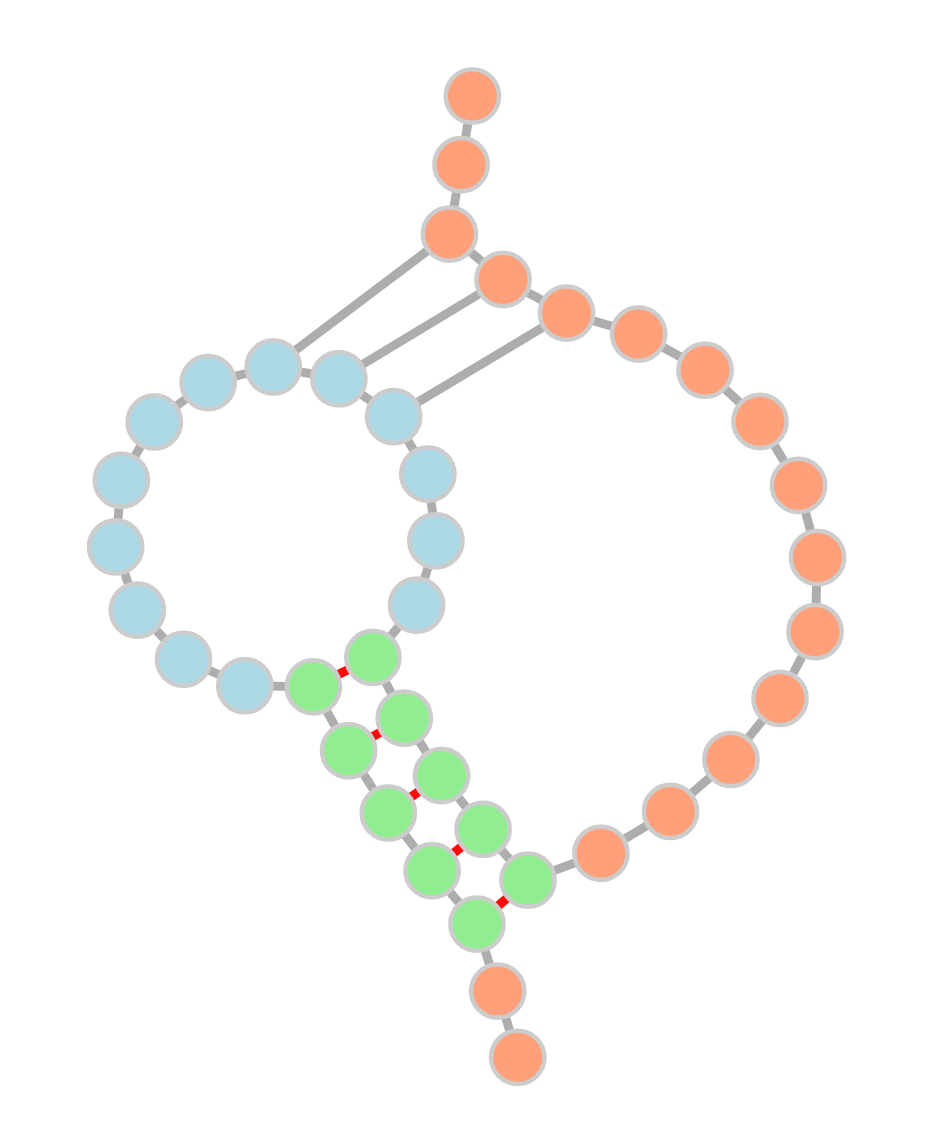
\includegraphics[width=0.8\textwidth]{pic/intro/rnahtype.png}
		\caption{A simple H-type (hairpin) pseudoknot.
		}\label{fig:htype:a}
	\end{subfigure}%
	\begin{subfigure}[t]{0.7\textwidth}
		\centering
		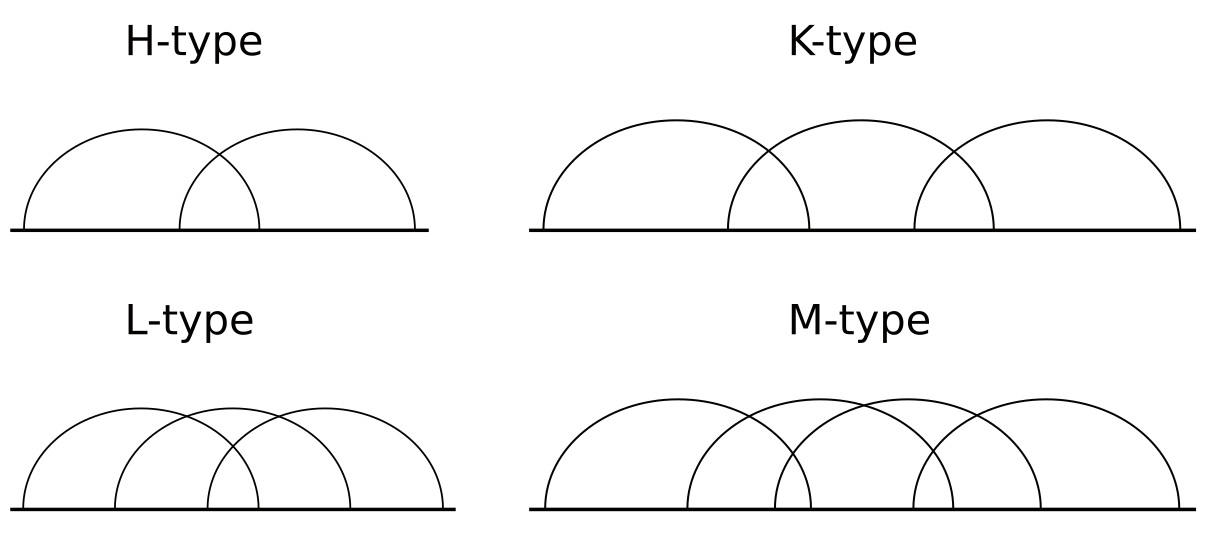
\includegraphics[width=\textwidth]{pic/intro/notmine/kucharik2016_fig1mod.png}
		\caption{More common pseudoknot types. The simplified H-type arc diagram can be visualized as \emph{stretching} \textbf{(a)} into a straight line.
		}\label{fig:htype:b}
	\end{subfigure}
	\caption[Some Common Pseudoknot Types]{
		\begin{enumerate*}[label={(\alph*)}, font={\bfseries}]
			\item An H-type pseudoknot. The dot-bracket notation \seqsplit{\textbf{\texttt{..(((((.......[[[...)))))..........]]]..}}} requires additional types of brackets in order to remain unambiguous.
			\item More types of pseudoknots, modified after \parencite{kucharik_pseudoknots_2016}. Both the H-type and K-type (kissing hairpin) pseudoknot are bi-secondary in the terminology of \parencite{haslinger_rna_1999}.
		\end{enumerate*}
	}\label{fig:htype}
\end{figure}

Aside from the complexity of arbitrary pseudoknots, integrating pseudoknots into the nearest-neighbor model is intricate since their energy contribution tends to be influenced by tertiary interactions \parencite{liu_fluorescence_2010}.

Nevertheless, the free energy of pseudoknots is often modelled similar to nested loop types by considering stacks of base pairs to be stabilizing and the enclosed loops as destabilizing \parencite{gultyaev_approximation_1999}.
While the former is straightforward, the latter is not exactly covered by the nearest-neighbor model.

Still,  the approach for multiloops in nested structures (see \autoref{eq:multi}) inspires a common approximation for pseudoknots. 
The destabilizing effect of a pseudoknot is approximated as the sum of a constant penalty (or initiation cost), a penalty depending on the number of enclosed unpaired nucleotides, and a penalty depending on the adjacent base pairs of the pseudoknot, i.e. the number of the participating crossing base pair stacks \parencite{dirks_partition_2003}.
For an H-type pseudoknot where only two stacks of base pairs are involved, computing this approximation is relatively simple.
Yet, even for K-type pseudoknots, some form of recursion is necessary.
A partition function algorithm of complexity $O(N^5)$ has been devised based on this approximation and is  available in \texttt{NUPACK} \parencite{dirks_partition_2003, zadeh_nupack_2011}.

Then again, for structures containing few and simple pseudoknots, the McCaskill algorithm for nested structures (see \autoref{par:theory:partfunc}) could be sufficient. 
Base pair probabilities obtained from it indicate possible pseudoknots, as was observed by Gaspin and Westhof and applied to \textit{Tetrahymena} by Mathews \parencite{gaspin_interactive_1995, mathews_using_2004}.

In the context of this work, secondary structures with pseudoknots are referred to as \emph{crossing} structures to emphasize the distinction to nested structures or disambiguate where necessary.

\end{document}
